\chapter{Testovanie založené na požiadavkách}
\label{requirements_based_testing}
Alebo aj requirement-based testing\footnote{\url{https://www.tutorialspoint.com/software_testing_dictionary/requirements_based_testing.htm}} je testovanie v ktorom sú testovacie prípady, dáta a podmienky založené na požiadavkách, takže testovanie založené na požiadavkách overuje, že testovaný softvér odpovedá požiadavkám.

\paragraph{Fázy testovania založeného na požiadavkách:}
\begin{itemize}
	\item definícia kritérii pokrytia,
	\item návrh testovacích prípadov,
	\item spustenie testov
	\item overenie výsledkov testov
	\item overenie pokrytia testov
	\item zaznamenanie nájdených chýb
\end{itemize}

Táto kapitola predstavuje rôzne požiadavky na testy a kritéria pokrytia, keďže návrh testovacích prípadov je priamo závislý na zvolenom kritériu pokrytia -- cieli testovania.


\section{Kritéria pokrytia}
\label{krietria_pokrytia}
Testovacia sada by sa mala tvoriť na základe predom predom zvoleného kritéria pokrytia s cieľom dosiahnuť 100\% pokrytia. 
Kritérium pokrytia definujú požiadavky na testy, test requirements (TR).
Množina požiadavkou na testy daného kritéria pokrytia môže byť väčšia než testovacia sada spĺňajúca pokrytie.
Jeden testovací prípad môže uspokojiť/pokryť niekoľko testovacích požiadavkou.
Existujú rôzne kritéria pokrytia zaoberajúcimi sa rôznými artefaktmi a sú rôzne silné.

\begin{definition}
Kritérium $C_1$ zahŕňa kritérium $C_2 \,(C_1 > C_2)$, práve vtedy, keď každá testovacia sada splňajúca kritérium $C_1$ tiež spĺňa kritérium $C_2$.
\end{definition}

\section{Testovanie založené na prechode grafom}
\todo{Rozdelenie do kapitol, usporiadanie}\\
Graf je jedna z najpouživanejších štruktúr pre abstrakciu, hlavne preto, lebo je dobre definová, veľmin názorná a je jednoduché ňom niečo jasne vyjadriť.
V testovaní poznáme niekoľko typov grafu, každý z nich testuje systém iným spôsobom~\cite{graph_testing}:
\begin{itemize}
	\item \textbf{Control flow graph (CFG)} -- graf toku riadenia: zachytáva informácie o tom, ako je v programe predávané riadenie.
	\item \textbf{Data flow graph} -- graf toku dát: modifikuje CFG pridaním informácii o dátových tokov.
	\item \textbf{Dependency graph} -- graf súvislostí: zachytáva dátové súvislosti, alebo súvislosti riadenia programu medzi príkazmi programu
	\item \textbf{Cause-effect graph} -- graf príčin a následkov: modeluje vzťahy medzi vstupnými podmienkami -- príčinami (causes) a výstupnými podmienkami -- následkami (effects).
\end{itemize}

Aj keď každý tento graf testuje funkcionatlitu SUT iným spôsobom a v tejto práci je ďalej vysvetlený graf toku riadenia a graf toku dát, postup pri testovaní založenom na prechode grafu je rovnaký:
\begin{enumerate}
	\item Vytvorenie modelu grafu: \\
		Aké informácie bude graf obsahovať a ako ich budeme reprezentovať.
	\item Zvoliť požiadavky na testy: \\
		Aké požiadavky musia byť splnené.
	\item Výber ciest grafu, ktoré pokryjú zvolené požiadavky.
	\item Odvodenie dát, aby mohli byť vybrané cesty spustené.
\end{enumerate}

\begin{figure}[H]
	\centering
	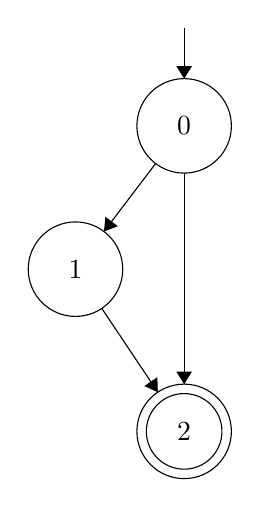
\begin{tikzpicture}[scale=0.2]
		\tikzstyle{every node}+=[inner sep=0pt]
		\draw [black] (34.9,-7.1) circle (3);
		\draw (34.9,-7.1) node {$0$};
		\draw [black] (28,-16.2) circle (3);
		\draw (28,-16.2) node {$1$};
		\draw [black] (34.9,-26.5) circle (3);
		\draw (34.9,-26.5) node {$2$};
		\draw [black] (34.9,-26.5) circle (2.4);
		\draw [black] (33.09,-9.49) -- (29.81,-13.81);
		\fill [black] (29.81,-13.81) -- (30.69,-13.47) -- (29.9,-12.87);
		\draw [black] (29.67,-18.69) -- (33.23,-24.01);
		\fill [black] (33.23,-24.01) -- (33.2,-23.06) -- (32.37,-23.62);
		\draw [black] (34.9,-0.9) -- (34.9,-4.1);
		\fill [black] (34.9,-4.1) -- (35.4,-3.3) -- (34.4,-3.3);
		\draw [black] (34.9,-10.1) -- (34.9,-23.5);
		\fill [black] (34.9,-23.5) -- (35.4,-22.7) -- (34.4,-22.7);
	\end{tikzpicture}
	\caption{Príklad jednoduchého grafu.}
\end{figure}

\subsection*{Pojmy z testovania založenom na prechode grafu}
\label{pojmy_cfg}
Tak ako pri pojmoch z testovanie~\ref{pojmy_testovanie} je potrebné definovať si pojmy, ktoré budú použité v nasledujúcich kapitolách práce:
\begin{description}
	\item\textbf{Cesta} v grafe ($path \subseteq N^+$) je neprázdna sekvencia uzlov [$n_1, n_2, \ldots, n_M$], taká, že každá dvojica susedných uzlov tvorí hranu v danom grafe:
		\begin{center}
			$(n_i, n_i + 1) \in E, 1 \leq i \leq M$
		\end{center}
	\item \textbf{Dĺžka cesty} je dána počtom hrán.
	\item \textbf{Testovacia cesta} začína niektorým počiatočným uzlom a končí v niektorom z koncových uzlov.
	\item \textbf{Podcesta cesty} $p$ je súvislý podreťazec daných uzlov.
	\item \textbf{Stopa (trace)} je taká cesta CFG, ktorá je realizovateľná testovaným subjektom.
	\item \textbf{Beh programu (run)} je stopa začínajúca v počiatočnom uzle a končiaca v koncovom uzle, pričom CFG odpovedá celému programu.
	\item Uzol je \textbf{syntaktický dosiahnuteľný (reachable)} z uzlu $n_i$, ak existuje cesta z uzlu $n$ do uzlu $n_i$.
	\item Uzol je \textbf{sémanticky dosiahnuteľný} z uzlu $n_i$, ak existuje nejaká stopa z uzlu $n$ do uzlu $n_i$.
	\item \textbf{Jednoduchá cesta} (Simple path) je taká cesta, v ktorej sa žiadny uzol neopakuje. Výnimkou je cesta, ktorá začína aj končí v rovnakom uzle.
	\item \textbf{Hlavná/primárna cesta} (Prime path) je taká jednoduchá cesta, ktorá nie je podcestou inej jednoduchej cesty, to znamená, že to je najdlhšia jednoduchá cesta.
	\item \textbf{Path (T)} pre testovaciu sadu T je množina ciest, respektíve stôp, ktoré sú spúšťané testovacími prípadmi z T.
\end{description}

\subsection{Riadiace toky}
Control flow graph (CFG) -- graf toku riadenia je orientovaný graf, v ktorom uzly reprezentujú základné bloky (basic blocks) a hrany reprezentujú cesty toku riadenia.
\begin{definition}
	\textbf{Control flow graph (CFG)} je čtvorica $\mathbf{G = (N, N_0, N_f, E)}$, kde:
\begin{itemize}
	\item $N$ je konečná množina uzlov,
	\item $N_0 \subseteq N, N_0 \neq \emptyset$, je neprázdna množina počiatočných uzlov,
	\item $N_f \subseteq N$ je množina koncových uzlov,
	\item $E \subseteq N \times N$ je množina hrán.
\end{itemize}
	\label{def:cfg}
\end{definition}
Pozn. Existujú rozšírené definície (napríklad s ohodnotením hrán).

\begin{description}
	\item \textbf{Základný blok} (basic block) je postupnosť maximálneho počtu príkazov, pre ktoré platí, že: 
		\begin{itemize}
			\item vstupných bod (riadenia) je na prvom príkaze, 
			\item výstupný bod riadenia je na poslednom príkaze a 
			\item príkazy sa vykonávajú vždy sekvenčne v poradí danom postupnosťou.
		\end{itemize}
		\label{def:basic_block}
\end{description}
Základný blok môže obsahovať príkaz pre vetvenie iba na konci.
Každý z uzlov $n_0$ až $n_3$ na obrázku \ref{fig:cfg_example} je základný blok.

\begin{figure}[H]
	\begin{subfigure}{0.4\linewidth}
		\centering
		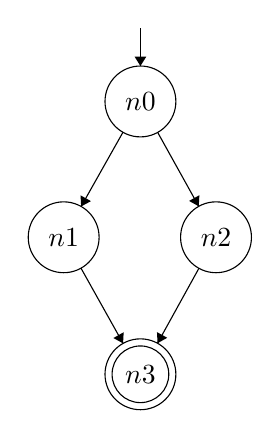
\begin{tikzpicture}[scale=0.15]
			\tikzstyle{every node}+=[inner sep=0pt]
			\draw [black] (34.9,-14.2) circle (3);
			\draw (34.9,-14.2) node {$n0$};
			\draw [black] (28.4,-25.7) circle (3);
			\draw (28.4,-25.7) node {$n1$};
			\draw [black] (41.3,-25.7) circle (3);
			\draw (41.3,-25.7) node {$n2$};
			\draw [black] (34.9,-37.3) circle (3);
			\draw [black] (34.9,-37.3) circle (2.4);
			\draw (34.9,-37.3) node {$n3$};
			\draw [black] (33.42,-16.81) -- (29.88,-23.09);
			\fill [black] (29.88,-23.09) -- (30.71,-22.64) -- (29.83,-22.15);
			\draw [black] (36.36,-16.82) -- (39.84,-23.08);
			\fill [black] (39.84,-23.08) -- (39.89,-22.14) -- (39.02,-22.62);
			\draw [black] (29.87,-28.32) -- (33.43,-34.68);
			\fill [black] (33.43,-34.68) -- (33.48,-33.74) -- (32.61,-34.23);
			\draw [black] (39.85,-28.33) -- (36.35,-34.67);
			\fill [black] (36.35,-34.67) -- (37.17,-34.21) -- (36.3,-33.73);
			\draw [black] (34.9,-8) -- (34.9,-11.2);
			\fill [black] (34.9,-11.2) -- (35.4,-10.4) -- (34.4,-10.4);
		\end{tikzpicture}
	\end{subfigure} 
	\quad
	\begin{subfigure}{0.4\linewidth}
		\centering
		\begin{algorithm}[H]
			\DontPrintSemicolon
			\LinesNotNumbered
			\SetNlSty{textbf}{}{:}

			\nlset{n0} \eIf{predicate()}{
				\nlset{n1} statement1(); \\
			}{
				\nlset{n2} statement2(); \\
			} 
			\nlset{n3}
		\end{algorithm}
	\end{subfigure}
	\caption{Jednoduchý control flow graf}
	\label{fig:cfg_example}
\end{figure}

\subsection*{Kritéria pokrytia riadiacich tokov}
\label{kriteria_cfg}
Požiadavky na testy v CFG môžme vyjadriť ako požiadavok na prechod hranou, alebo navštívenie vybraných uzlov -- obidve požiadavky zahrnujú cestu.

\begin{description}
	\item Kritérium pokrytia uzlov, \textbf{Node Coverage (NC)} vyžaduje, aby požiadavky na test obsahovali každý syntaktický dosihnuteľný uzol.
		%TODO: pridat, alebo nie?
		%\begin{definition}
		%	Testovaci sada T splňuje pokrytie uzlov (NC) na grafu G, práve vtedy, keď pre každý syntaktický dosiahnuteľný uzol $n \in N$ existuje cesta $p \in path(T)$ obsahujúca uzol $n$.
		%\end{definition}
	\item Kritérium pokrytia hran, \textbf{Edge Coverage (EC)} vyžaduje, aby požiadavky na test obsahovaly každú syntakticky dosiahnuteľnú cestu o dĺžke 0, alebo 1\footnote{Požiadavok na cestu dĺžky 0 z uzlu $n$ odpovedá požiadavku na prechod uzlom $n$ -- špeciálny prípad grfau bez hrán}.
	\item Kritérium pokrytia párov hrán, \textbf{Edge-Pair Coverage (EPC)} vyžaduje, aby požiadavky na test obsahovali každú syntaktiky dosiahnuteľnú cestu o dĺžke najviac 2.
	\item Kritérium pokrytia hlavných ciest, \textbf{Prime Path Coverage (PPC)} vyžaduje, aby požiadavky na testy obsahovali všetky hlavné cesty. Príklad je na obrázku~\ref{fig:ppc_coverage}.
\end{description}
Porovnanie kritérii pokrytia riadiacich tokov je na obrázku ~\ref{fig:coverage}.

\begin{figure}[H]
	\centering
	\begin{subfigure}{0.4\linewidth}
		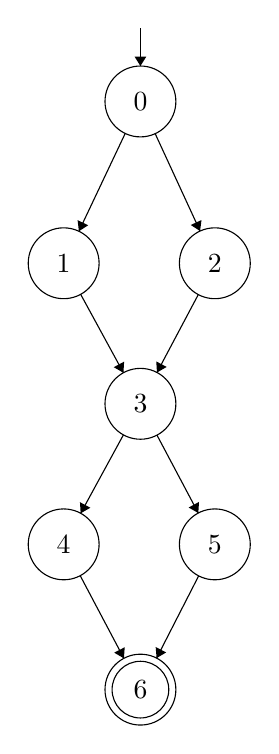
\begin{tikzpicture}[scale=0.15]
			\tikzstyle{every node}+=[inner sep=0pt]
			\draw [black] (34.9,-7.1) circle (3);
			\draw (34.9,-7.1) node {$0$};
			\draw [black] (28.4,-20.8) circle (3);
			\draw (28.4,-20.8) node {$1$};
			\draw [black] (34.9,-32.7) circle (3);
			\draw (34.9,-32.7) node {$3$};
			\draw [black] (41.2,-20.8) circle (3);
			\draw (41.2,-20.8) node {$2$};
			\draw [black] (28.4,-44.6) circle (3);
			\draw (28.4,-44.6) node {$4$};
			\draw [black] (41.2,-44.6) circle (3);
			\draw (41.2,-44.6) node {$5$};
			\draw [black] (34.9,-56.9) circle (3);
			\draw (34.9,-56.9) node {$6$};
			\draw [black] (34.9,-56.9) circle (2.4);
			\draw [black] (33.61,-9.81) -- (29.69,-18.09);
			\fill [black] (29.69,-18.09) -- (30.48,-17.58) -- (29.58,-17.15);
			\draw [black] (29.84,-23.43) -- (33.46,-30.07);
			\fill [black] (33.46,-30.07) -- (33.52,-29.13) -- (32.64,-29.6);
			\draw [black] (34.9,-0.9) -- (34.9,-4.1);
			\fill [black] (34.9,-4.1) -- (35.4,-3.3) -- (34.4,-3.3);
			\draw [black] (36.15,-9.83) -- (39.95,-18.07);
			\fill [black] (39.95,-18.07) -- (40.07,-17.14) -- (39.16,-17.56);
			\draw [black] (39.8,-23.45) -- (36.3,-30.05);
			\fill [black] (36.3,-30.05) -- (37.12,-29.58) -- (36.24,-29.11);
			\draw [black] (33.46,-35.33) -- (29.84,-41.97);
			\fill [black] (29.84,-41.97) -- (30.66,-41.5) -- (29.78,-41.03);
			\draw [black] (36.3,-35.35) -- (39.8,-41.95);
			\fill [black] (39.8,-41.95) -- (39.86,-41.01) -- (38.98,-41.48);
			\draw [black] (29.8,-47.25) -- (33.5,-54.25);
			\fill [black] (33.5,-54.25) -- (33.57,-53.31) -- (32.68,-53.77);
			\draw [black] (39.83,-47.27) -- (36.27,-54.23);
			\fill [black] (36.27,-54.23) -- (37.08,-53.75) -- (36.19,-53.29);
		\end{tikzpicture}
	\end{subfigure} \quad
	\begin{subfigure}{0.4\linewidth}
		\begin{eqnarray*}
			 path(t_1) = [0, 1, 3, 4, 6] \\
			 path(t_2) = [0, 2, 3, 5, 6] \\
			 path(t_3) = [0, 1, 3, 5, 6] \\
			 path(t_4) = [0, 2, 3, 4, 6] \\
		\end{eqnarray*}
		\bigskip
		\begin{tabular}{ |l|c|c|c|  } 
			\hline
			Testovacia sada & NC & EP & EPC \\ 
			\hline
			\hline
			$T_1 = \{t_1\}$ & $\times$ & $\times$ & $\times$ \\ 
			\hline
			$T_2 = \{t_2\}$ & $\times$ & $\times$ & $\times$ \\ 
			\hline
			$T_3 = \{t_1, t_2\}$  & \checkmark & \checkmark & $\times$ \\ 
			\hline
			$T_4 = \{t_1, t_2, t_3, t_4\}$  & \checkmark & \checkmark & \checkmark \\ 
			\hline
		\end{tabular}
	\end{subfigure}
	\caption{Porovnanie kritérii pokrytia}
	\label{fig:coverage}
\end{figure}

\begin{figure}[H]
	\begin{subfigure}{\linewidth}
		\centering
		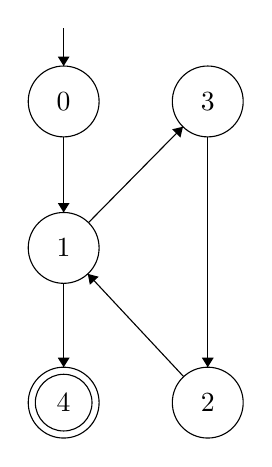
\begin{tikzpicture}[scale=0.15]
			\tikzstyle{every node}+=[inner sep=0pt]
			\draw [black] (34.9,-7.1) circle (3);
			\draw (34.9,-7.1) node {$0$};
			\draw [black] (34.9,-19.5) circle (3);
			\draw (34.9,-19.5) node {$1$};
			\draw [black] (34.9,-32.6) circle (3);
			\draw (34.9,-32.6) node {$4$};
			\draw [black] (34.9,-32.6) circle (2.4);
			\draw [black] (47.1,-7.1) circle (3);
			\draw (47.1,-7.1) node {$3$};
			\draw [black] (47.1,-32.6) circle (3);
			\draw (47.1,-32.6) node {$2$};
			\draw [black] (34.9,-10.1) -- (34.9,-16.5);
			\fill [black] (34.9,-16.5) -- (35.4,-15.7) -- (34.4,-15.7);
			\draw [black] (34.9,-22.5) -- (34.9,-29.6);
			\fill [black] (34.9,-29.6) -- (35.4,-28.8) -- (34.4,-28.8);
			\draw [black] (34.9,-0.9) -- (34.9,-4.1);
			\fill [black] (34.9,-4.1) -- (35.4,-3.3) -- (34.4,-3.3);
			\draw [black] (37,-17.36) -- (45,-9.24);
			\fill [black] (45,-9.24) -- (44.08,-9.46) -- (44.79,-10.16);
			\draw [black] (47.1,-10.1) -- (47.1,-29.6);
			\fill [black] (47.1,-29.6) -- (47.6,-28.8) -- (46.6,-28.8);
			\draw [black] (45.06,-30.4) -- (36.94,-21.7);
			\fill [black] (36.94,-21.7) -- (37.12,-22.62) -- (37.86,-21.94);
		\end{tikzpicture}
	\end{subfigure}
	\bigskip
	\begin{subfigure}{\linewidth}
		\centering
		\begin{eqnarray*}
			PP = \{[0, 1, 2], [0, 1, 3, 4], [1, 3, 4, 1],
			[3, 4, 1, 3], [3, 4, 1, 2]\} \\
			path(t_1) = [0, 1, 2] \\
			path(t_2) = [0, 1, 3, 4, 1, 3, 4, 1, 2] \\
			T_2 = \{ t_1, t_2\} \text{ splňuje PPC.}
		\end{eqnarray*}
	\end{subfigure}
	\caption{Príklad prime path coverage}
	\label{fig:ppc_coverage}
\end{figure}

%TODO: cyklomatická zložitosť?
\subsection{Dátové toky}
Aby sme mohli sledovať dátové toky programu, potrebujeme v grafe (CFG) zaznamenať ako sa pristupuje k dátam.
Pre zjednodušenie sú dáta brané ako neznáme hodnoty v pomenovaných úložiskách.
Zaujíma nás \texttt{tok dát}, teda z ktorých úložísk sa \textbf{číta} a do ktorých sa \textbf{zapisuje}.
Nezaujímajú nás konštanty, ani výraza, teda čo sa s dátami deje.

\todo{Takto? alebo ako to je v \ref{def:cfg}}\\
Rozšírená definícia CFG:
\begin{definition}
	\textbf{CFG pre analýzu dátových tokov} je n-tica: 
	\begin{center}
		$\mathbf{G = (N, N_0, N_f, E, V, D, U)}$
	\end{center}
	kde:
	\begin{itemize}
		\item $N, N_0, N_f a E$ sú uzly a hrany podľa definície~\ref{def:cfg},
		\item $V$ je konečná množina premenných,
		\item $D: N \rightarrow 2^V$ je funkcia priradzujúca každému uzlu množinu premenných, ich hodnota je v uzle definová (tzv. \texttt{def funkcia}) a
		\item $U: N \rightarrow 2^V$ je funkcia priradzujúca každému uzlu množinu premenných, ktoré sú v danom uzle čítané (tzv. \texttt{use funkcia}).
	\end{itemize}
\end{definition}

Používame nasledujúce funkcie:
\begin{description}
\item \textbf{def(n) = \{$v_1, v_2, \ldots, v_n$\}}, ktorá hovorí, že uzol $n$ definuje hodnoty pre premenné $v_1, v_2, \ldots, v_n$ (zapisuje do premenných):
	\begin{itemize}
		\item premenná sa vyskytuje na ľavej starane priradenia,
		\item premenná je predaná odkazom do podprogramu,
		\item premenná je fomrálny parameter podprogramu.
	\end{itemize}
\item \textbf{use(n) = \{$v_1, v_2, \ldots, v_n$\}}, ktorá hovorí, že uzol $n$ používa hodnoty premenných $v_1, v_2, \ldots, v_n$ (číta hodnoty premenných):
	\begin{itemize}
		\item premenná sa vykytuje na pravej stane priradenia,
		\item premenná sa vyskytuje vo výraze pre podmienený skok,
		\item premenná je predána hodnotou podprogramu,
		\item premenná je čítaná návratová hodnoto podprogramu.
	\end{itemize}
\end{description}

\begin{figure}[H]
	\begin{subfigure}{0.5\linewidth}
		\centering
		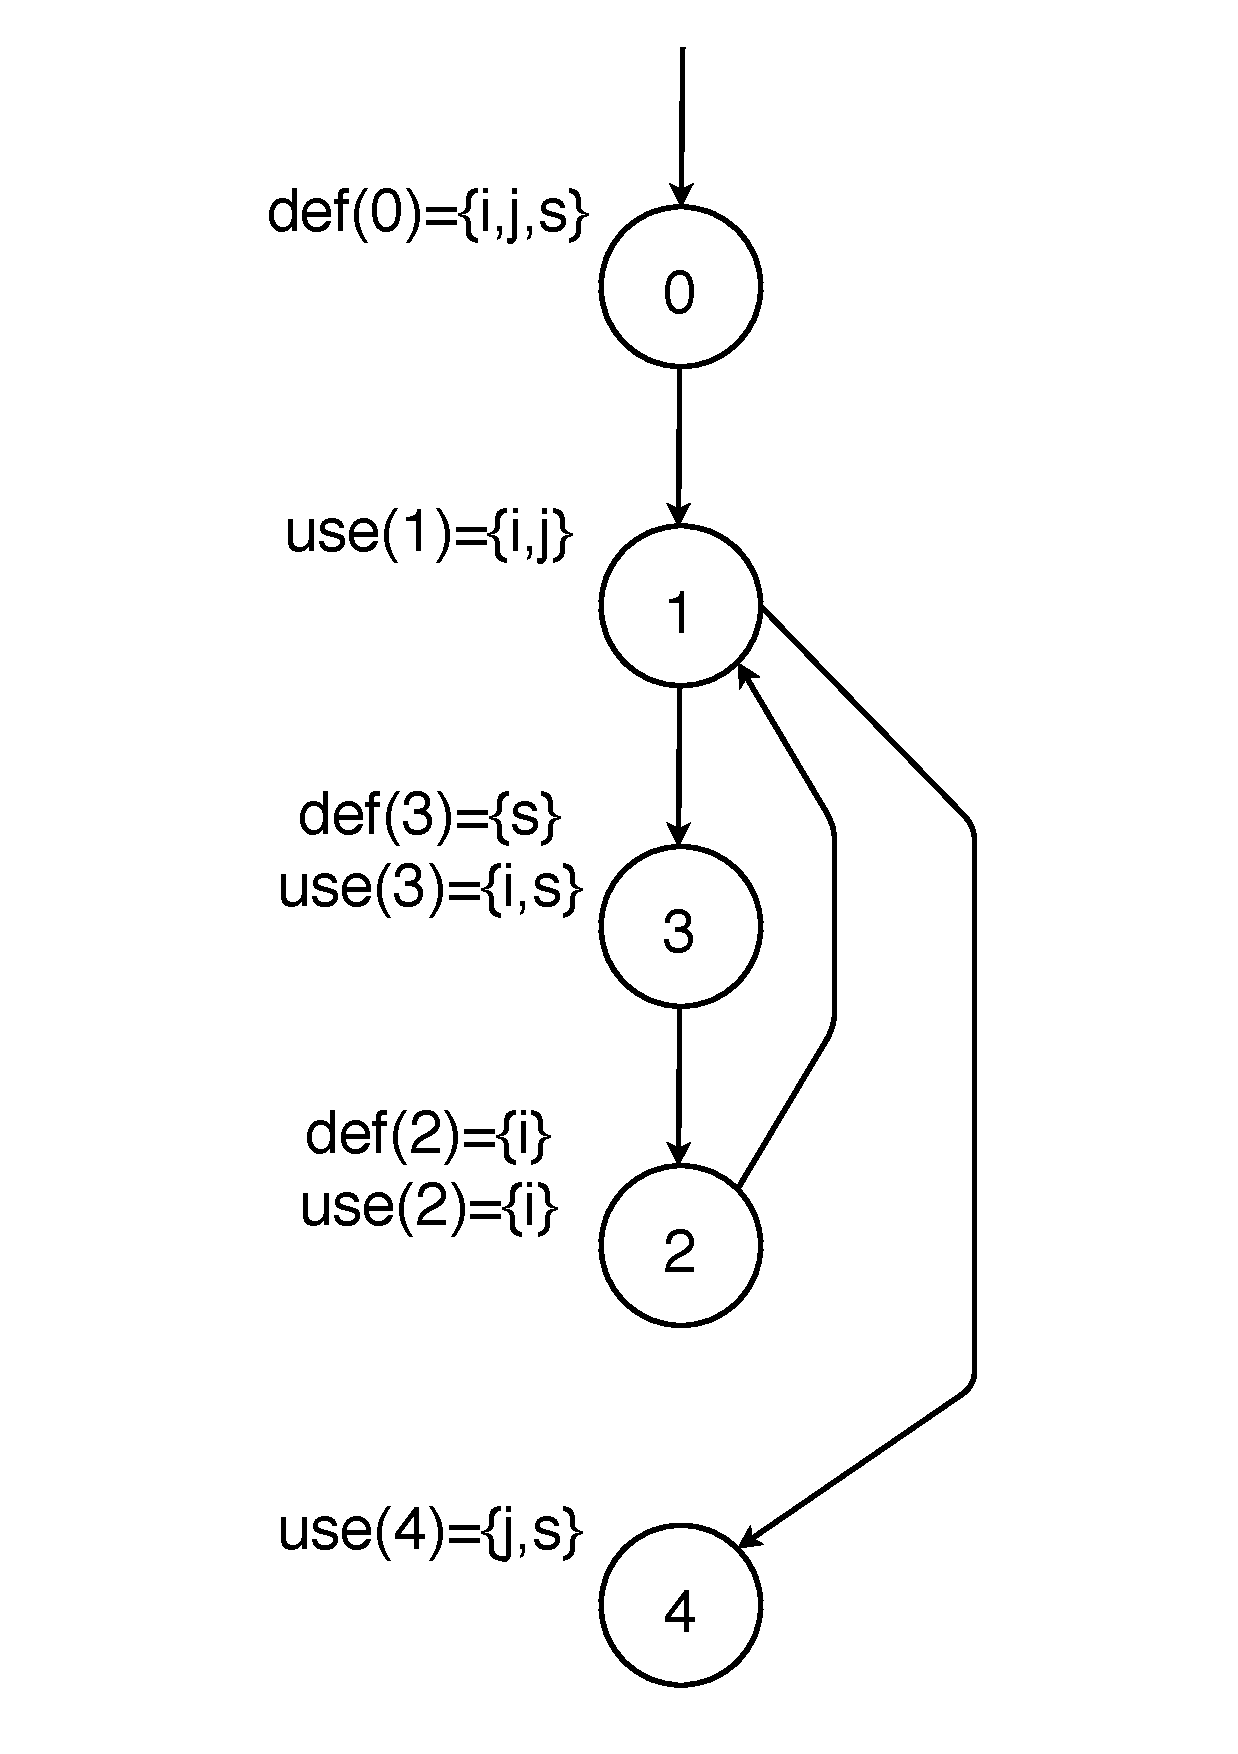
\includegraphics[width=0.8\linewidth]{obrazky/cfg_def_use.pdf}
	\end{subfigure}
	\quad
	\begin{subfigure}{0.5\linewidth}
		\centering
		\begin{algorithm}[H]
			\DontPrintSemicolon
			\LinesNotNumbered
			\SetNlSty{textbf}{}{:}
			\nlset{0} j = get\_size(); \\
			\For{(i = 0, s = 0; \\
				\nlset{1}i < j; \\
				\nlset{2}i++)}{
				\nlset{3}s += foo(i);
			}
			\nlset{4}bar(s/j)
		\end{algorithm}
	\end{subfigure}
	\caption{Príklad CFG s def a use funkciami.}
\end{figure}

Hodnoty premenných sú prenášané z miesta definíce na miesto použitia.
Tieto páry nazývame \textbf{du-pairs} (definition-use pairs).

Zaujímajú nás cesty medzi definíciou a použitím pre danú premennú:
Cesta \textbf{du-path} je jednoduchá cesta~\ref{pojmy_cfg} \texttt{v} CFG [$n_i, \ldots, \_j$], pre ktorú platí:
\begin{itemize}
	\item $v \in$ def($n_i$) -- prvý uzel definuje hodnotu premennej,
	\item $v \in$ use($n_j$) -- posledný uzel premennú používa,
	\item $v \not\in$ def($n_k$), pre $i < k < j$ -- žiadny uzel medzi prvým posledným premennu nedefinuje.
\end{itemize}
Cesta je jednoduchá, aby bol počet ciest konečný.
Podmienka cesty byť jednoduchá má za následok, že premenná môže byť na danej ceste použitá niekoľkokrát.


Testovacie kritéria pre dataflow budú definované ako množina ciest du-path.
Preto definujeme zoskupenie týchto množín:
\begin{description}
	\item \textbf{def-pair du($n_i, n_j, v$)} je množina všetkých ciest du-path pre premennú $v$, ktoré začínajú v uzle $n_i$ a končia v uzel $n_j$.

	\item \textbf{def-path du($n_i, v$)} je množina všetkých ciest du-path pre premennú $v$, ktoré začívajú v uzle $n_i$, resp. du($n_i, v$) = $\cup_{n_j}$ du($n_i, n_j, v$).
\end{description}

\subsection*{Kritéria pokrytia dátových tokov}
\begin{description}
	\item Kritérium pokrytia všetkých definícii \textbf{All-Defs Coverage (ADC)} vyžaduje, aby pre každú množinu cies du(n, v) požiadavky na testy obsahovaly aspoň jednu cestu z danej množiny.
		\begin{itemize}
			\item Požiadavky na testy musia obsahovať aspoň jednu cestu pre každú premennú a pre každú jej definiciu.
		\end{itemize}
		Toto kritérium testuje, že každé priradenie premennej dáva pre nejaké jej použitie zmysel.

	\item Kritérium pokrytia všetkých použizí \textbf{All-Uses Coverage (AUC)} vyžaduje, aby pre každú množinu ciest du ($n_i, n_j, v$) požiadavky na testy obsahovali aspoň jednu cestu z danej množiny.
		\begin{itemize}
			\item Požiadavky na testy musia obsahovať aspoň jednu cestu z každej dvojice def-use.
		\end{itemize}
		Toto kritérium testuje testuje, či každá dvojica priradenia a následného použitia dáva zmysel.

	\item Kritérium pokrytia všetkých du-ciest \textbf{All-du-Paths Coverage (ADUPC)} vyždaduje, aby požiadavky na testy obsahovali každú cestu z každej množiny ciest du($n_i, n_j, v$).
		\begin{itemize}
			\item Požiadavky na testy musia obsahovať všetky možné cesty zo všetkých definíc premenných ku všetkým možných použitia.
		\end{itemize}
		Toto kritérium testuje, či neexistuje nezmyselné dátové spojenie medzi definíciou a použitím premennej.
\end{description}

\begin{figure}[H]
	\begin{subfigure}{0.5\linewidth}
		\centering
		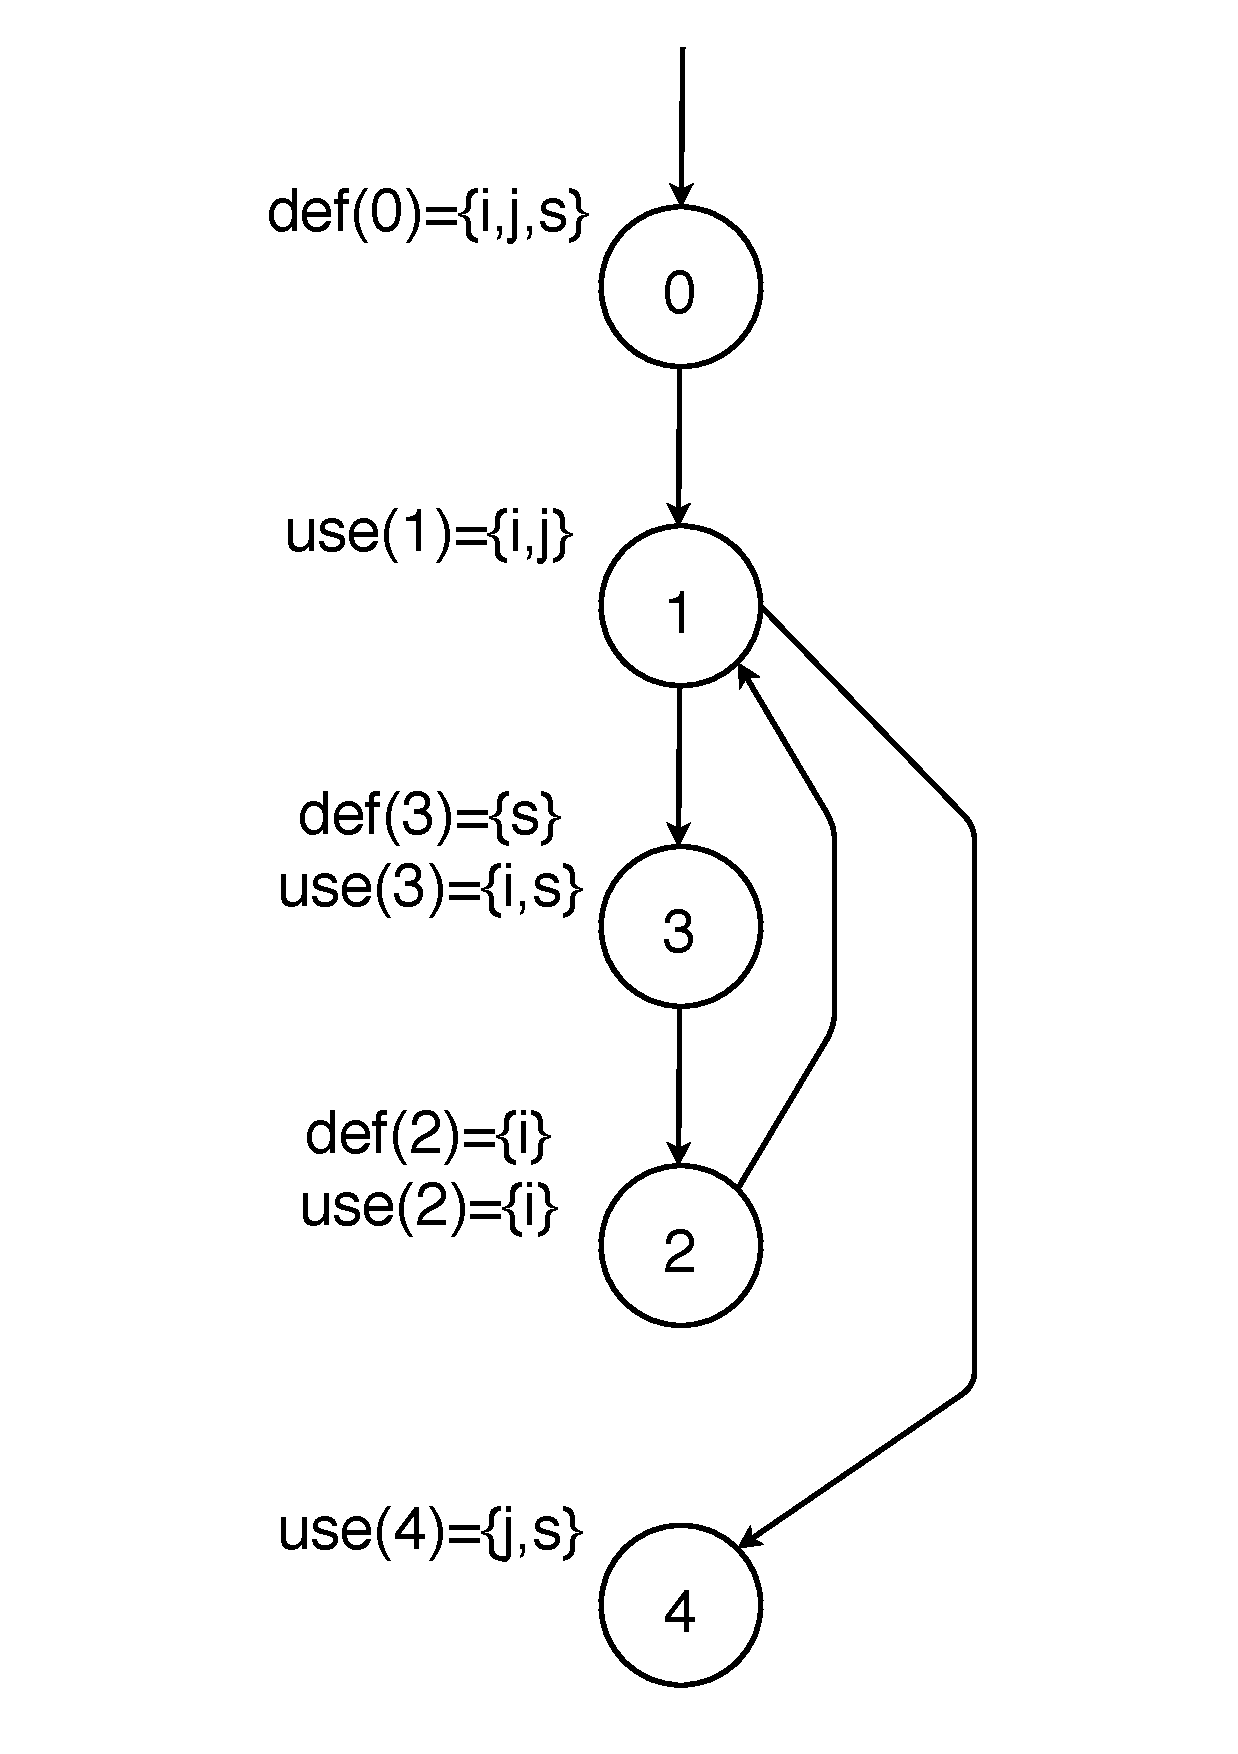
\includegraphics[width=0.8\linewidth]{obrazky/cfg_def_use.pdf}
	\end{subfigure}
	\quad
	\begin{subfigure}{0.5\linewidth}
		du(0, 3, s) = \{[0, 1, 3]\} \\
		du(0, 4, s) = \{[0, 1, 4]\} \\
		du(3, 3, s) = \{[3, 2, 1, 3]\} \\
		du(3, 4, s) = \{[3, 2, 1, 4]\} \\

		du(0, s) = \{[0, 1, 3], [0, 1, 4]\} \\
		du(3, s) = \{[3, 2, 1, 3], [3, 2, 1, 4]\}
	\end{subfigure}
	\bigskip
	\begin{subfigure}{\linewidth}
		\centering
		\begin{tabular}{ |l|c|c|c|  } 
			\hline
			Testovacia sada pre s\footnote{Iba ako demonštrácia. Splniteľnosť ADC, AUC, ADUPC sa totiž vzťahu ku všetkým premenným}& ADC & AUC & ADUPC \\ 
			\hline
			\hline
			$T_1 = \{[0, 1, 4]\}$ & $\times$ & $\times$ & $\times$ \\ 
			\hline
			$T_2 = \{[0, 1, 3, 2, 1, 4]\}$ & \checkmark & $\times$ & $\times$ \\ 
			\hline
			$T_3$ $=$ $\{[0, 1, 4],$ $[0, 1, 3, 2, 1, 3, 2, 1, 4]\}$ & \checkmark & \checkmark & \checkmark \\ 
			\hline
		\end{tabular}
	\end{subfigure}
	\caption{Príklad pokrytia dátových tokov.}
\end{figure}

\begin{figure}[H]
	\begin{subfigure}{0.5\linewidth}
		\centering
		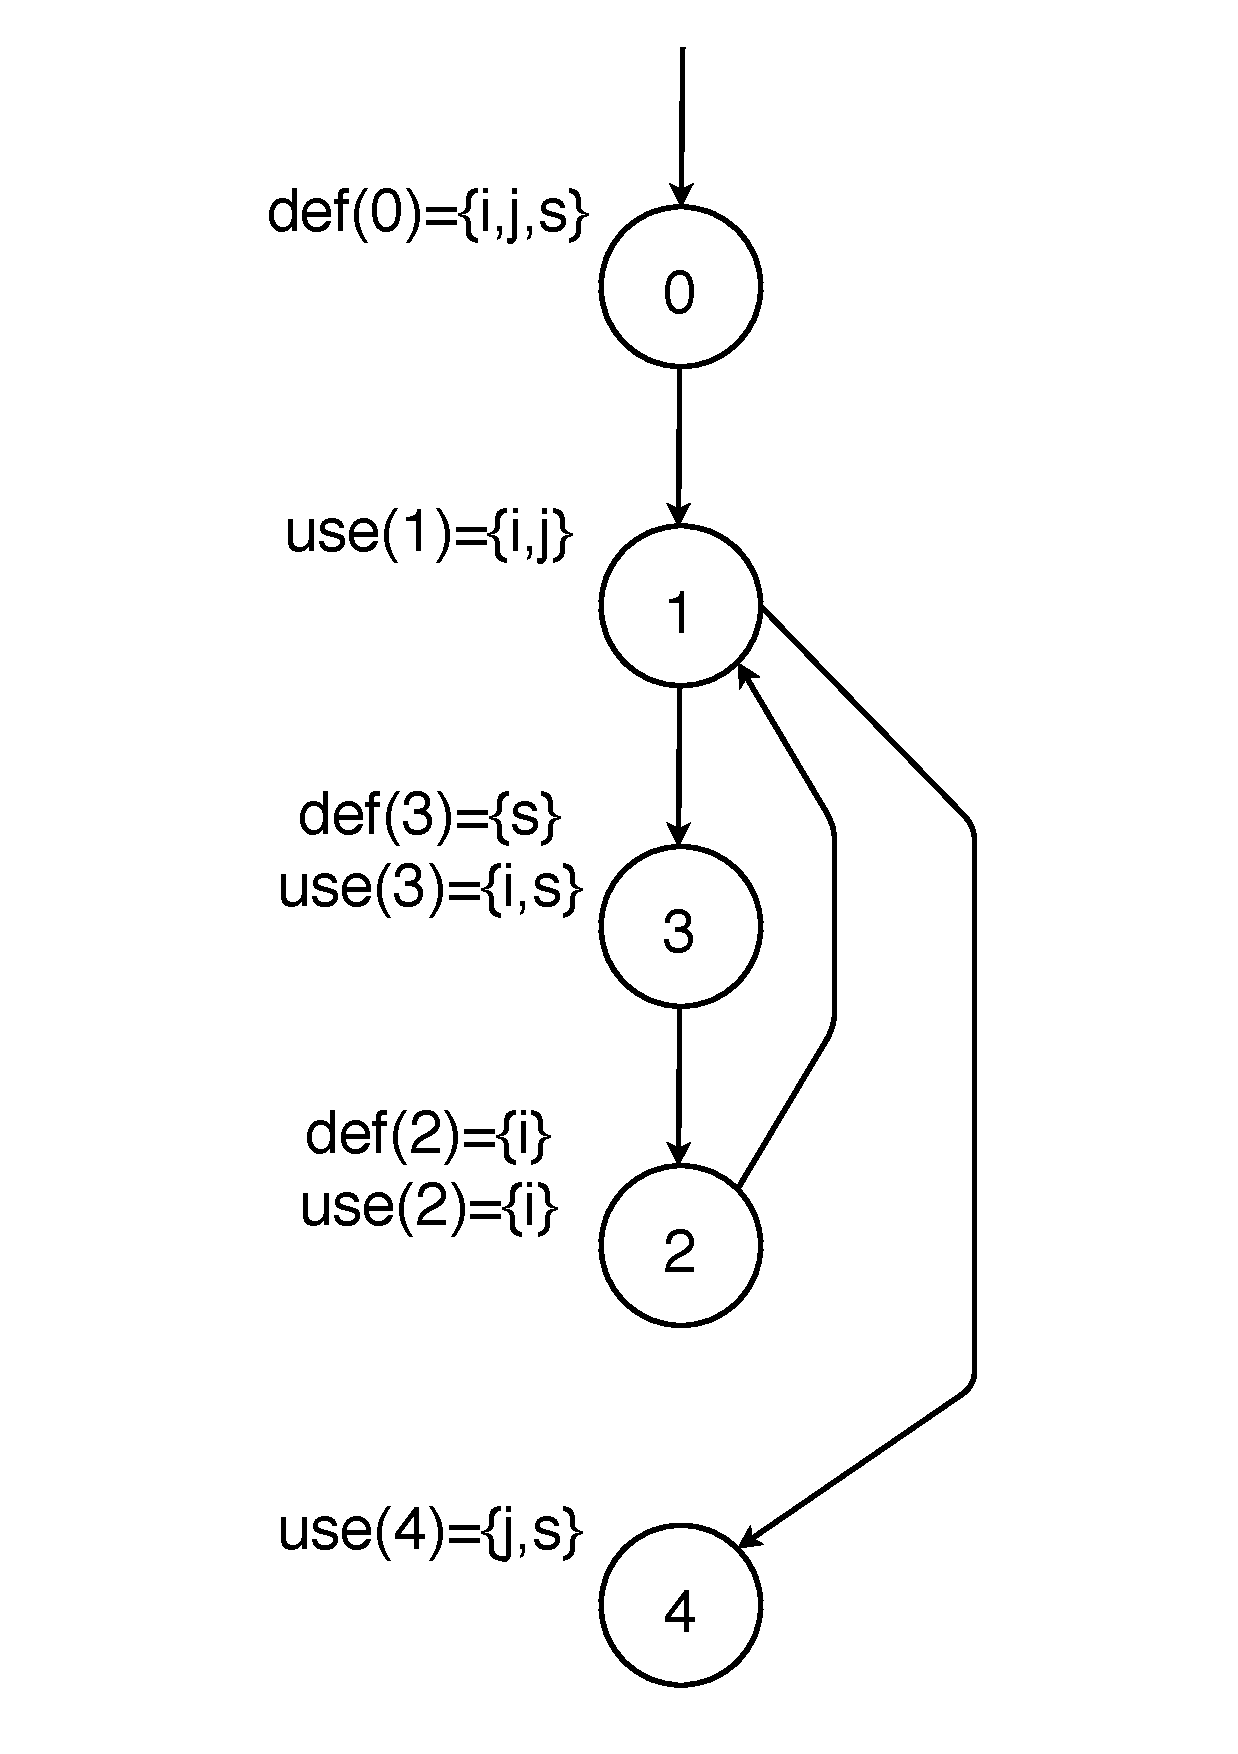
\includegraphics[width=0.8\linewidth]{obrazky/cfg_def_use.pdf}
	\end{subfigure}
	\begin{subfigure}{0.5\linewidth}
		\centering
		\begin{tabular}{ |c| } 
			\hline
			All-defs (ADC) \\
			\hline
			$T_1 = \{[0, 1, 3, 4, 6]\}$ \\
			\hline
		\end{tabular}
		\bigskip

		\begin{tabular}{ |c| } 
			\hline
			All-uses (AUC) \\
			\hline
			$T_2 = \{[0, 1, 3, 4, 6], [0, 2, 3, 5, 6]\}$ \\
			\hline
		\end{tabular}
		\bigskip

		\begin{tabular}{ |c| } 
			\hline
			All-du-paths (ADUPC) \\
			\hline
			$T_2 = \{[0, 1, 3, 4, 6],$ \newline$[0, 2, 3, 5, 6], [0, 1, 3, 5, 6], [0, 2, 3, 4, 6]\}$ \\
			\hline
		\end{tabular}
	\end{subfigure}
	\caption{Príklad rozšíreného CFG a testovacích sád.}
\end{figure}

\begin{figure}[H]
	\begin{subfigure}{0.4\linewidth}
		\centering
		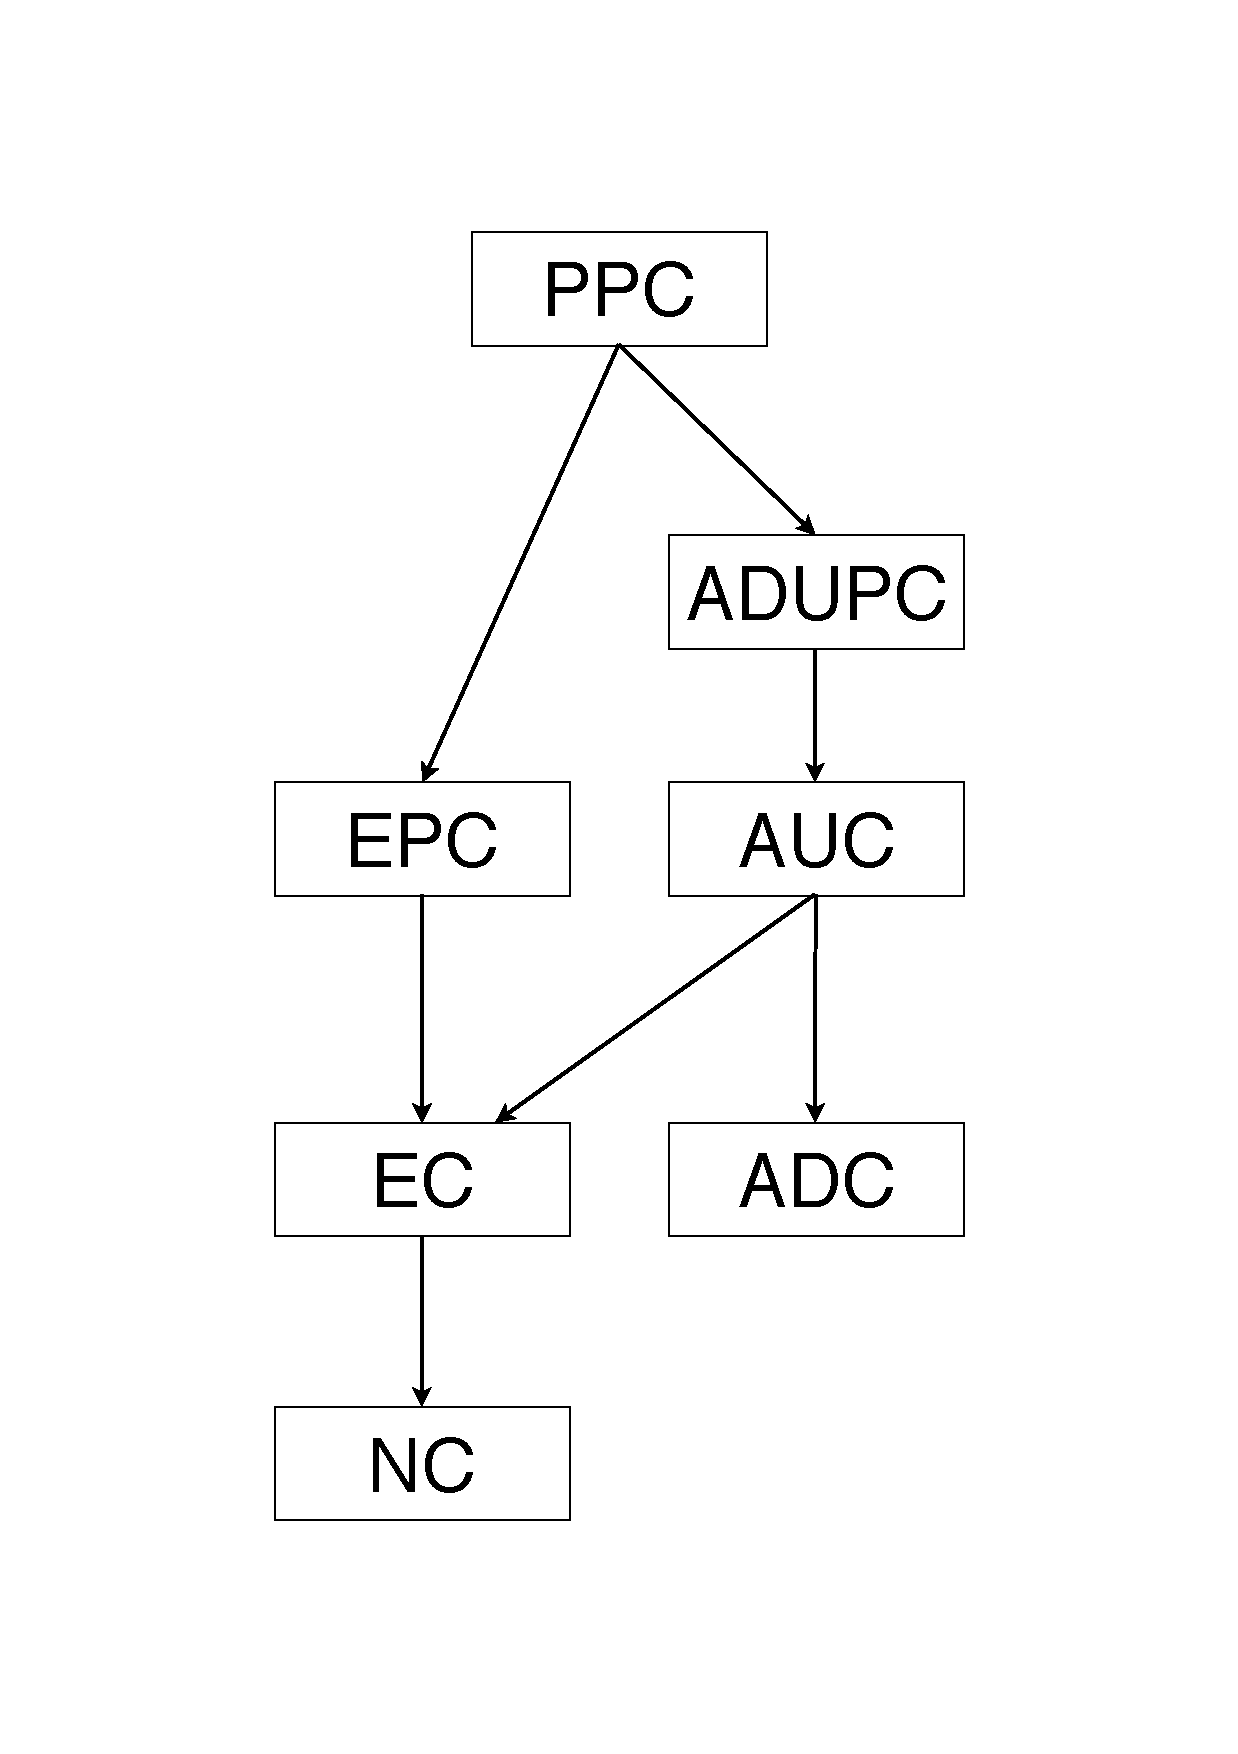
\includegraphics[width=\linewidth]{obrazky/vztah_kriterii.pdf}
	\end{subfigure}
	\quad
	\begin{subfigure}{0.4\linewidth}
		\centering
		\begin{flushleft}
			\large
			PPC -- Prime Path Coverage \\
			\medskip
			EPC -- Edge-Pair Coverage \\
			\medskip
			EC -- Edge Coverage \\
			\medskip
			NC -- Node Coverage \\
			\medskip
			ADUPC -- All-du-Paths Coverage \\
			\medskip
			AUC -- All-Uses Coverage \\
			\medskip
			ADC -- All-Defs Coverage \\
		\end{flushleft}
	\end{subfigure}
	\caption{Vzťah kritérii pokrytia.}
\end{figure}

%\subsection{Logické výrazy}
%\todo{testovanie logických výrazov}
% netreba to tam
\section{Vstupné domény}
\label{vstupne_domeny}
\textbf{Vstupná doména} (doména vstupu, priestor, input space) je množina všetkých vstupov systému.
Môžo to byť:
\begin{itemize}
	\item vstupné parametre metód,
	\item globálne, alebo statické premenné,
	\item vstupy od užívateľa, atgumenty programu,
	\item objekty reprezentujúce aktuálny stav systému.
\end{itemize}
Vstupná doména je rozdelená na menšie celky(bloky, regióny, časti)\footnote{V matematike je to rozklad na ekvivalenčné triedy}, ktoré obsahujú rovnako užitočné hodinoty z pohľadu testovania.
\begin{table}{H}
	\centering
	\begin{tabular}{ | c | c | c | c | c | }
		\hline
		$b_1$ & $b_2$ & $b_3$ & $b_4$ & $b_5$ \\
		\hline
		$x < 0$ & $x > 0$ & $x = 0$ & isinf(x) & isnan(x) \\
		\hline
	\end{tabular}
	\caption{Príklad rozkladu jednorozmernej domény.}
\end{table}

Niektoré behy programu je možné zoskupiť do rovnakej kategórie -- pre rôzne vstupy sa program chová rovnako.
Cieľom je otestovať všetky takéto kategórie, pričom z každej kategórie stačí vybrať iba jeden testovací prípad.

\subsection*{Rozklad vstupných domén}
\label{rozklad_domen}
Každá správna charakteristika definuje rozklad domény (q), ktorý musí spĺňať nasledujúce podmienky:
\begin{itemize}
	\item Jednotlivé bloky rozkladu ($B_q$) musiac byť vzájomne disjunktné, nesmú sa prekrývať:
		\begin{center}
			$b_i \cap b_j = \emptyset, i \not = j, b_i, b_j \in B_q$
		\end{center}
	\item Vštky bloky dohromady musia byť kompletné, rozklad musí zahrňovať celú doménu:
		\begin{center}
			$\underset{b \in B_q}{\bigcup} b = D$
		\end{center}
\end{itemize}
\todo{Napíš nejaké vysvetlenie a tak}\\

\subsection*{Model vstupných domén}
\label{model_domen}
\textbf{Model vstupnej domény} (input domain model) je abstrakcia vstupov testovaného systému.
Tester popisuje štruktúru modelu vstupných doméch pomocou charakteristik.
Pre každú charakteristiku rozkladá domény na jednotlivé bloky.
Každý blok predstavuje množinu hodnôt vstupov SUT.
Tieto hodnoty sú z hľadiska testov považované za rovnocenné.

\subsection*{Kritéria pokrytia vstupných domén}\
\label{kriteria_pokrytia_domen}
\begin{itemize}
	\item Kritérium pokrytia všetkých kombinácii \textbf{All Combinations Coverage (ACoC)} vyžaduje, aby TR obsahovali všetky kombinácie blokov zo všetkých charakteristík.
		\todo{príklad}\\
	\item Kritérium pokrytia každého bloku \textbf{Each Choice Coverage (ECC)} vyžaduje, aby TR obsahovali každý blok re každú charakteristiku.
		\todo{príklad}\\
	\item Kritérium pokrytia všetkých párov blokov \textbf{Pair-Wise Coverage (PWC)} vyžaduje, aby TR obsahovali každý blok každej charakteristiky a každý pár blokov každý z inej charakteristiky.
		\todo{príklad}\\
	\item PWC je možné zobecniť na \textbf{T-Wise Coverage} (nie dvojice, aby T-tice blokov).
	\item Kritérium pokrytia bázových blokov \textbf{Base Choice Coverage (BCC)} vyžaduje, aby TR obsahovali kombinácie všetkých bázových blokov každej charakteristiky a každý jeden nebázový blok v kombinácii s bázovými blokmi.
		\todo{príklad}\\
\end{itemize}

\begin{figure}[H]
	\centering
	\begin{subfigure}{0.4\linewidth}
		\centering
		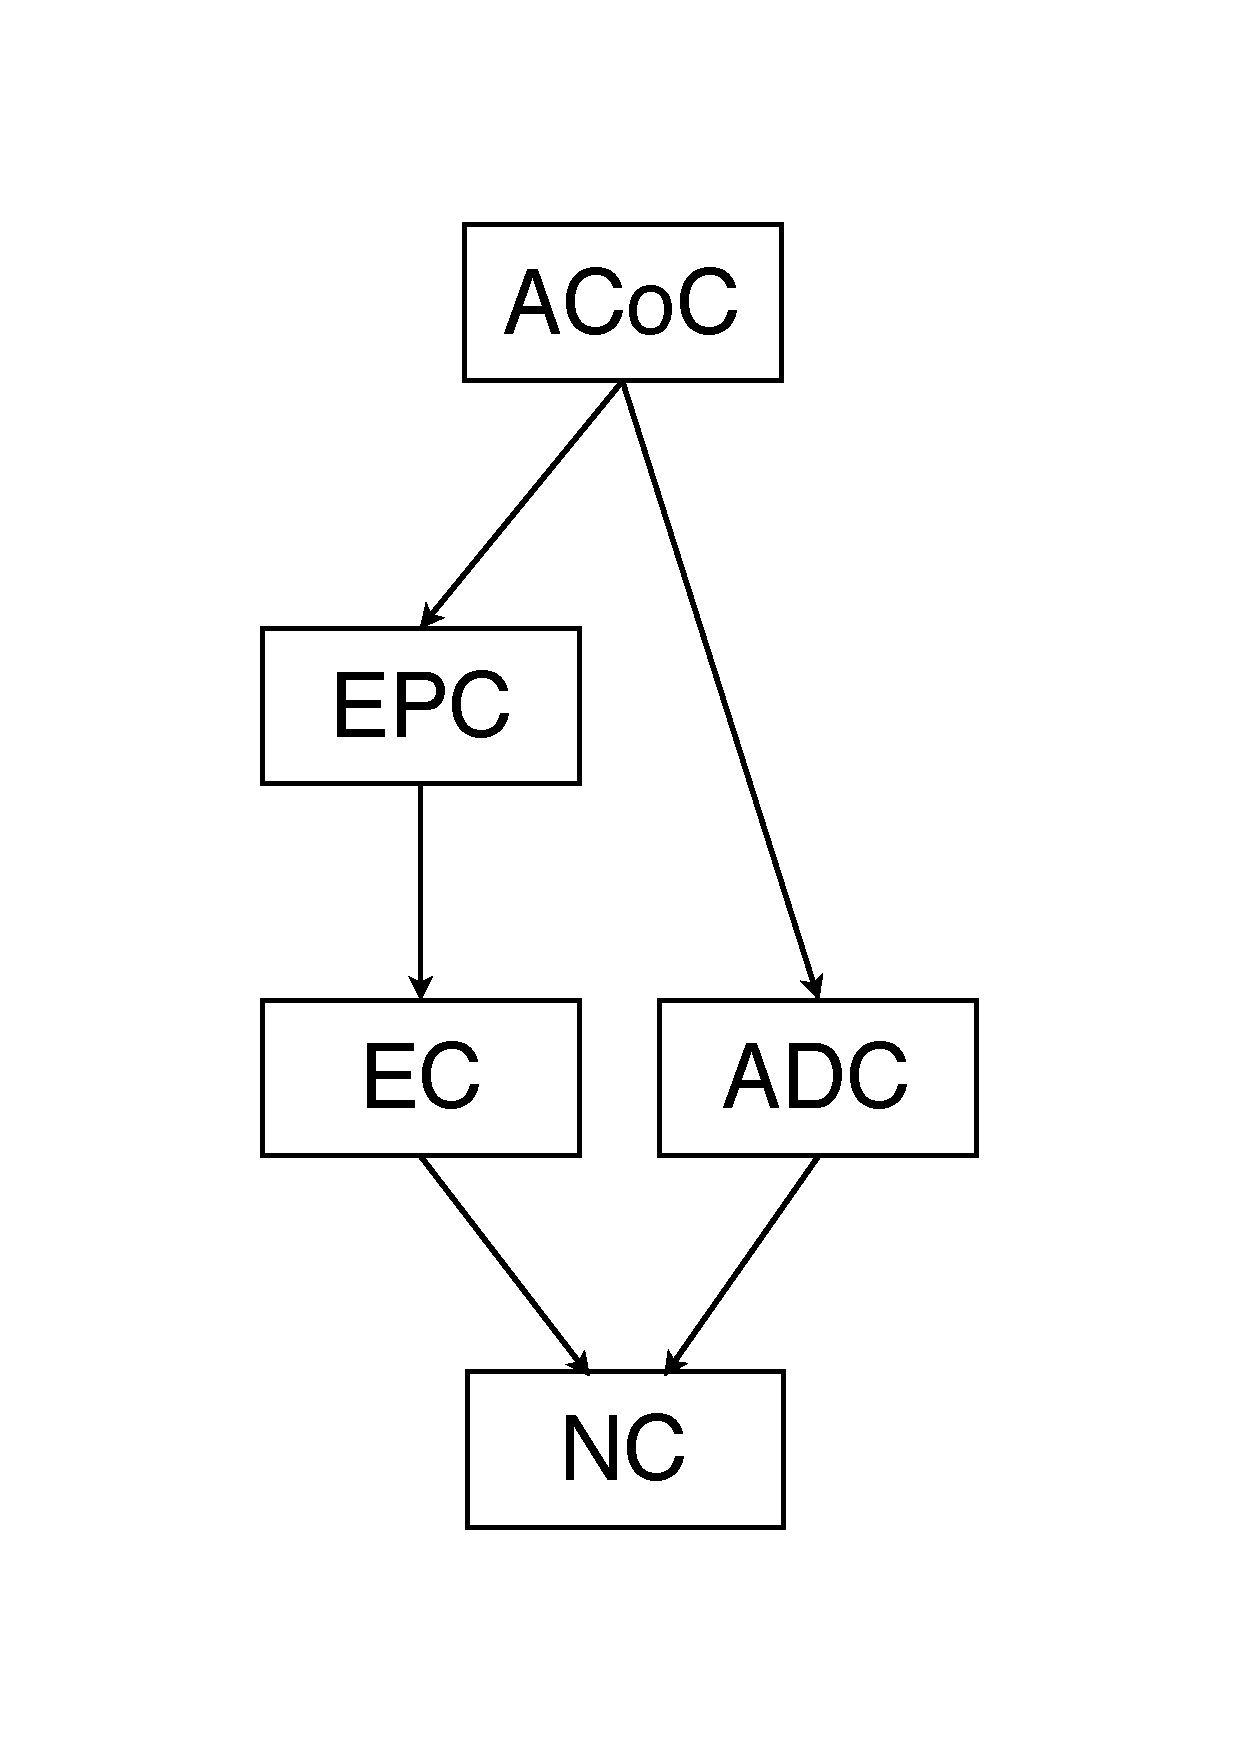
\includegraphics[width=\linewidth]{obrazky/vztah_kriterii_domen.pdf}
	\end{subfigure}
	\quad
	\begin{subfigure}{0.4\linewidth}
		\centering
		\begin{flushleft}
			\large
			ACoC -- All Combinations Coverage \\
			\medskip
			TWC -- T-Wise Coverage \\
			\medskip
			PWC -- Pair-Wise Coverage \\
			\medskip
			BCC -- Base Choice Coverage \\
			\medskip
			ECC -- Each Choice Coverage \\
		\end{flushleft}
	\end{subfigure}
	\caption{Vzťah kritérii pokrytia vstupných domén.}
\end{figure}

\section{Fixtures}
\label{fixtures}
Test fixture podľa vzoru XUnit\footnote{\url{http://xunitpatterns.com/}} je množina predpokladov alebo stavov potrebných na spustenie testu. Vývojár testov by mal pripraviť tieto podmienky pred spustením testy a po testy by mal SUT vrátiť do pôvodneho stavu~\cite{Beck}.

XUnit takisto definuje fázy testov:
\begin{itemize}
	\item Setup (príprava prostredia pre test),
	\item Exercise (spustenie SUT),
	\item Verify (overenie výsledkov),
	\item Teardown (vrátenie SUT do pôvodného stavu).
\end{itemize}
Test fixture sú teda všetky vstupné dáta pre SUT, aby bolo možné spustiť test opakovane a bez ohľadu na aktuálny kontext~\cite{Smrcka}.

\textbf{Test Double} (dvojník) je objekt, ktorý má reprezentovať pôvodný objekt na ktorom je SUT (a test) závislý.
\begin{itemize}
	\item Musí mať rovnaké rozhranie -- stačí aj podmnožina rozhrania využívaná SUT behom testu ak to jazyk dovoľuje.
	\item Nemal by mať ďalšie závislosti -- okrem tých, ktoré sú využívané SUT.
	\item Podľa schopností existuje niekoľko typov:
		\begin{itemize}
			\item Dummy -- existuje, ale nič nerobí,
			\item Stub -- vracia prednastavenú hodnotu,
			\item Spy -- sleduje a zaznamenáva,
			\item Mock -- sleduje, overuje, vracia,
			\item Shims -- upravuje kompilovaný kód za behu (run-time), aby injektoval s spúšťal metódy substituce (tzv. detour),
			\item Fakes -- takmer plnohodnotné náhrada (napríklad databáza v pamäti).
		\end{itemize}
\end{itemize}

V testovacej komunite sú najpoužívanejšie Stub a Mock objekty.
\begin{description}
	\item[Stubs]\
		\label{stub}
		\begin{itemize}
			\item Nezáleží na vstupoch, stále vráti preddefinovanú hodnotu (objekt).
			\item Nemôže spôsobiť zlyhanie testu.
			\item Vzor \texttt{State Verification\footnote{\url{http://xunitpatterns.com/State\%20Verification.html}}} -- overuje sa výsledný stav SUT.
		\end{itemize}
	\item[Mocks]
		\label{mock}
		\begin{itemize}
			\item Kontroluje vstupy a výstupné hodnoty posiela v závislosti na vstupných hodnotách.
			\item Môže spôsobiť zlyhanie testu.
			\item Vzor \texttt{Behavior Verification\footnote{\url{http://xunitpatterns.com/Behavior\%20Verification.html}}} -- overuje sa tiež vnútorné chovanie SUT.
		\end{itemize}
\end{description}
\todo{Čorknút obrázky k tým verifications} \\
